\section{Introduction}

\begin{frame}{Expérience}
    \begin{columns}
        \column{.6\textwidth}
        \begin{figure}
            \centering
            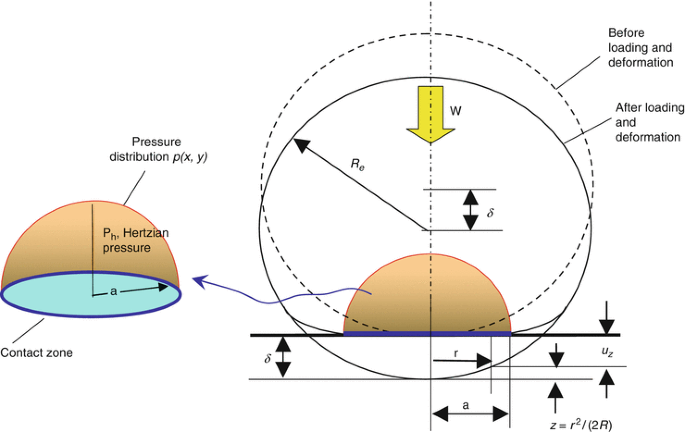
\includegraphics[width=0.95\textwidth]{contactHertzPhoto.png}
            \caption{Scema de notre expérience\cite{Wang2013}}
            \label{fig:wiki}
        \end{figure}
        \column{.4\textwidth}
        \begin{figure}
            \centering
            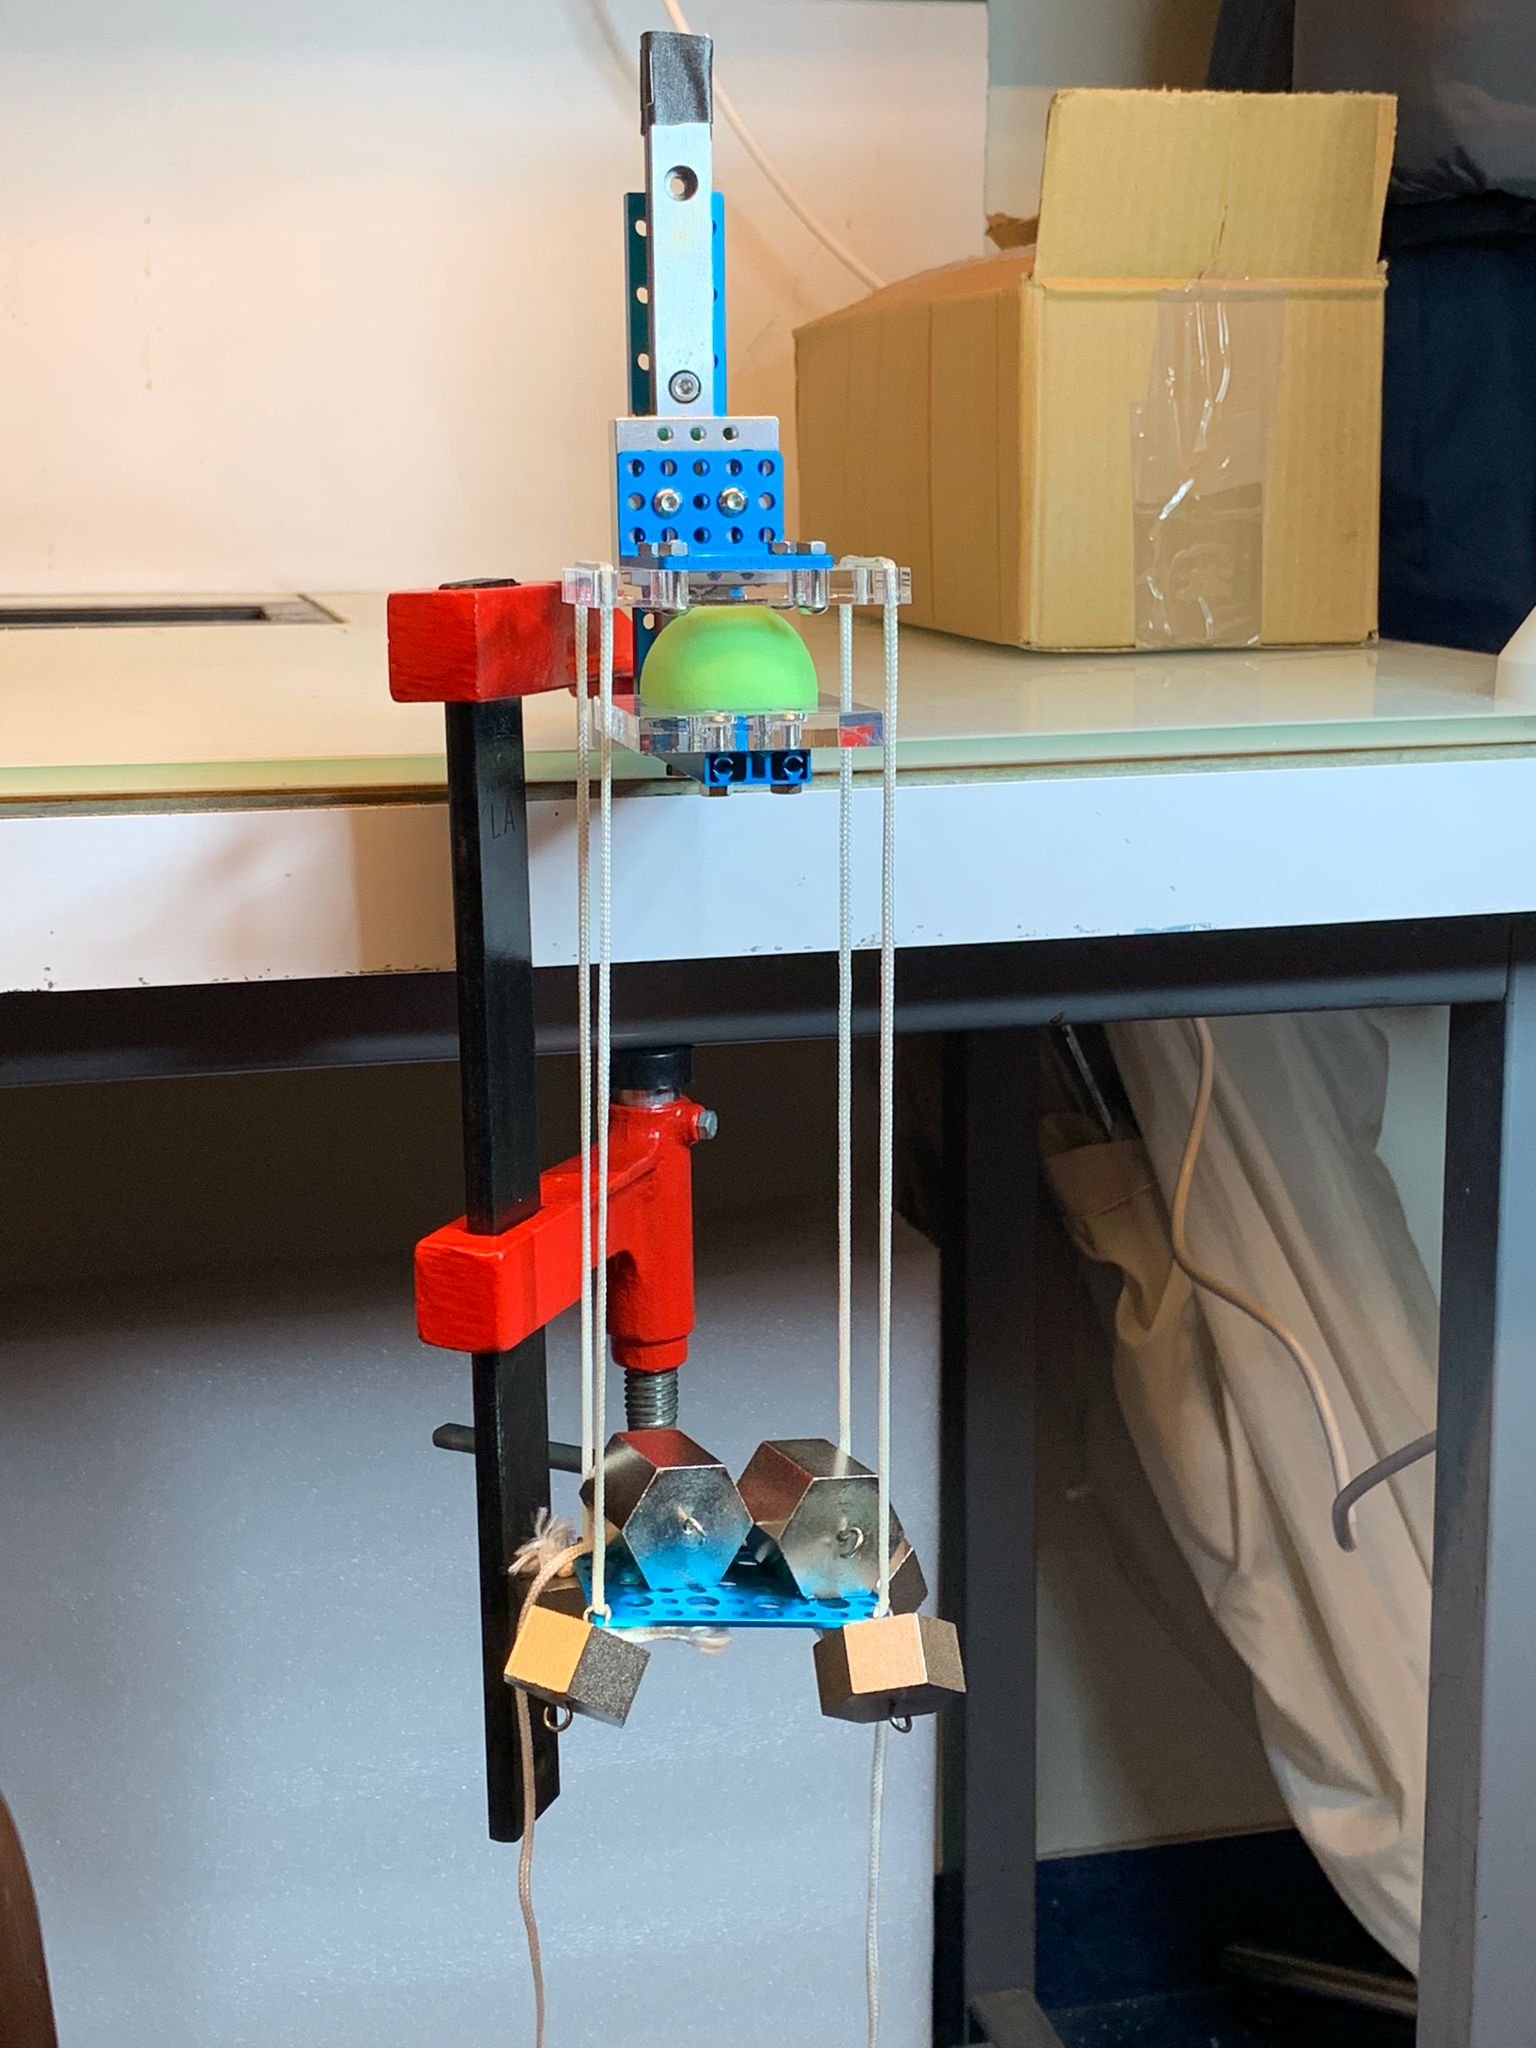
\includegraphics[height=0.7\textheight]{Figures/IMG-20221205-WA0025.jpg}
            \caption{Image de notre expérience}
            \label{fig:my_label}
        \end{figure}
    \end{columns}
\end{frame}

\begin{frame}{Les paramètres}
    \begin{itemize}
        \item Le diamètre (paramètre observable).
        \item Le poids.
        \item La masse.
        \item Module de Young.
        \item Rayon du sphère.
    \end{itemize}
    \begin{block}{Relation entre 5 paramètres dimensionnés}
        \begin{center}
            \(d_{allongé}=f(g,m,Y,r)\)
        \end{center}
    \end{block}
\end{frame}

\subsection{Théorème de Vaschy-Buckingham}
\begin{frame}{Théorème de Vaschy-Buckingham}
    \begin{columns}
        \column{.5\textwidth}
        \begin{itemize}
            \item 5 paramètres dimensionnés: d, g, m, Y, r.
            \item 3 dimensions: L, T, M.
            \item 2 nombres $\Pi$.
        \end{itemize}
        \column{.5\textwidth}
        \begin{block}{Nos nombre Pi's}   
            \begin{itemize}
                \item \(\Pi_1 = \frac{d_{allongé}}{r}\)
                \item \(\Pi_2 = \frac{Y}{g\cdot m\cdot r^{-2}}\)
            \end{itemize}
        \end{block}
    \end{columns}
\end{frame}
